\documentclass[twocolumn]{IEEEtran}
\usepackage{graphicx}
\usepackage{subcaption}
\usepackage{hyperref}

\begin{document}
\title{Enfoque CoEvolutivo al problema del Ladron Viajero}
\author{Angel David Corredor}
\date{}
\maketitle

\begin{abstract}
    Este articulo presenta una tecnica para resolver una formulación de el problema del
    ladron viajero (Traveling Thief Problem) usando un enfoque coevolutivo.
    Existen 2 poblaciones que resuelven separadamente los subproblemas de TTP
    pero trabajan juntos para solucionar el problema combinado usando el concepto de amigos.
    Finalmente se muestran los resultados obtenidos al aplicar esta tecnica. 
\end{abstract}

\section{Introducción}

El problema del ladron viajero es la combinación de 2 conocidos problemas de 
optimización: el agente viajero y el problema de la mochila (TSP y KP).
Al combinar estos problemas se vuelven interdependientes, de tal manera que resolver
alguno de los sub-problemas por separado no es efectivo, de tal manera que es necesario
considerar ambos problemas de manera conjunta.

A continuación se presenta la formulación de cada uno de los problemas.

\subsection{Problema del Agente viajero}

El problema del agente viajero es uno de los los problemas clasicos de optimizacion NP-hard.
En este problema se tienen $n$ ciudades y las distancias entre ellas estan dadas por una matriz
$D=d_{ij}$ ($d_{ij}$, la distancia entre las ciudades $i$ y $j$).
Tenemos un vendedor que debe visitar cada una de las ciudades exactamente una vez. Se asume que 
su velocidad de desplazamiento es constante ($v_c$) e intenta minimizar el tiempo que toma completar
el tour.
La funcion objectivo se define entonces como:

\begin{equation}
    f(\bar{x}) =
    \sum_{i=1}^{n-1} (t_{x_i,x_{i+1}})
    + t_{x_n,x_1},
    \bar{x}=(x_1,...,x_n)
\end{equation}

donde $\bar{x}$ representa un tour, el cual contiene cada una de las ciudades exactamente una vez
y $t_{x_i,x_{i+1}}$ es el tiempo de viaje entre $x_i$ y $x_{i+1}$ el cual se calcula como:

\begin{equation}
    t_{x_i,x_{i+1}} =
    \frac{d_{x_i,x_{i+1}}}{v_c}
\end{equation}

Claramente, $f$ es el tiempo total que toma completar el tour.
El objetivo es entonces encontrar el $\bar{x}$ que minimiza $f$.

\subsection{Problema de la mochila}
El problema de 
la mochila es otro problema de optimización NP-hard.
En este problema, se tienen $m$ items $I_1, ..., I_m$, cada uno de ellos con
un valor ($p_i$) y un peso ($w_i$) asignado.
Una persona quiere llenar su mochila tomando algunos de estos items.
La capacidad de la mochila esta limitada a $W$.
El problema se modela de la siguiente manera:

\begin{equation}
    maximize \; g(\bar{y}) =
    \sum_{i=1}^m p_iy_i, 
    \bar{y} = (y_1, ..., y_m)
\end{equation}

\begin{equation}
    subject \; to
    \sum_{i=1}^m w_iy_i \leq W
\end{equation}

donde $y_i \in \{0,1\}$ y $y_i = 1$ indica que se toma el objeto $i$ y
$g(y)$ es el valor total de los items tomados. 
El objetivo es maximizar $g$ con la restricción de que el peso total no puede exeder
la capacidad de la mochila.
El objetivo es tomar los items que maximizan la ganancia $g$, mientras que su peso
total no supera la capacidad de la mochila.

\subsection{Problema del Ladron Viajero}
Se formula entonces el problema del ladron viajero como una combinación de los problemas
anteriores, de manera que un ladron desea recorrer un número $n$ de ciudades, obteniendo
durante su viaje el mayor beneficio tomando unos items que estan en cada ciudad. 

Con el objetivo de interconectar estos dos problemas se añaden varios parámetros adicionales,
los cuales son:

\begin{itemize}
    \item La velocidad del viaje ($v_c$ en (2)) se relaciona al peso actual de la mochila.
    ($v_c = (v_{max} - W_c \frac{v_{max}-v_{min}}{W})$)
    donde $W_c$ es el peso actual de la mochila, $v_{max}$ y $v_{min}$
    son la maxima y miima velocidad del ladrón respectivamente, y
    $W$ es la capacidad máxima de la mochila. Notese que 
    el tiempo de viaje es calculado usando (2).
    De acuerdo a esta formulación la velocidad del ladron ($v_c$)
    disminuye cuando el peso de la mochila aummenta, ademas el ladron
    viaja a $v_{max}$ cuando la mochila esta vacia
    ($W_c=0$) y a $v_min$ cuando la mochila esta llena ($W_c=W$).

    \item El ladron rentó la mochila y debe pagar el restamo.
    La cuota de la mochila es de $\$R$ por unidad de tiempo.

\end{itemize}

    La función objetivo entonces en esta formulación de TTP es maximizar la siguiente función:

    \begin{equation}
        G(x,z) = g(z) - R*f(x,z)
    \end{equation}

    donde $g$ es el valor de los items tomados, $R$ es la renta de la mochila
    por unidad de tiempo, y $f$ es el tiempo total en recorrer las ciudades. $x$ y $z$ son el
    tour y los items a tomar (las soluciones de los subproblemas TSP y KP), respectivamente.
    Notese que el tiempo de viaje y el peso de los items están conectados a travez de los
    cambios en la velocidad del viaje. Por esto, la funcion $f$ necesita a $x$ y a $z$
    para calcular el tiempo total. Al mismo tiempo el valor total de los items tomados
    estan conectados al tiempo de viaje y el valor de la renta.

\section{Codificación del Problema}

Para resolver el problema se utilizarán 2 poblaciones independientes dedicadas a 
solucionar cada uno de los subproblemas, pero conectadas con un amigo en la otra población
como se plantea en COFRE, es decir una relación no transitiva.%Pendiente citación

Las poblaciones usadas son:

\subsection{Población TSP}
Se usa la codificación habitual de TSP, la cual es na permutación de $n$ elementos llamada tour
la cual representa el orden en que el viajero (o el ladrón) debe visiatar las ciudades.
Adicionalmente, cada individuo tiene un número que identifica su amigo en la población KP.

\subsection{Población KP}
Se usa la codificación habitual para el problema de la mochila, la cual es un 
arreglo de tamaño $m$ que representa la decision de tomar o no el item i-esimo.
Adicionalmente se tiene un número que identifica a su amigo en la población TSP (codificado en base 2).

\subsection*{Amigos}
Al calcular el rendimiento de un individuo de cualquiera de las poblaciones, es necesario identificar
a su amigo para poder hacer la evaluación de la función objetivo.
Este sistema hace que la evaluación sea no estacionaria, ya que ningún individuo tiene control
sobre los cambios que pueda sufrir su amigo ni hace cambio de amigo basado en el rendimiento de estos.

\section{Experimentación}
Partiendo de la definición de la función objetivo se configuran 2 algoritmos geneticos
independientes que evolucionan ambas poblaciones y se realizan cambios sobre el operador de
selección de padres para poder evaluar los cambios que esto conduce sobre los resultados obtenidos.

Se realizan entonces 2 experiementos en 2 instancias del problema TTP (eil51 n50 y eil76 n75),
contando cada uno de estos con 30 ejecuciones de los
algoritmos conjuntos, cada una de ellas con 100 generaciones de 100 individuos
(por población) cada una.

\section{Resultados}

\subsection{Selección Uniforme}
Se usa el operador de selección uniforme de padres para ejercer menos presion evolutiva
en este apartado, los resultados obtenidos se reflejan en la figura \ref{figure:51_random}
y la tabla \ref{table:results_rand}:

\begin{table}[htpb]
    \centering
    \begin{tabular}{|c|c|c|c|c|}
        \hline
        Problema & $\bar{x}$ & $\sigma_{\bar{x}}$ & mediana & $\sigma_{med}$ \\
        \hline
        eil51 n50 & -633926.81 & 1191789.64 & -239351.74 & 1257545.48 \\
        \hline
        eil76 n75 & -519887.5124 & 303620.9418 & -497407.7530 & 304544.1917 \\
        \hline
    \end{tabular}
    \caption{Resumen estadistico selección uniforme}
    \label{table:results_rand}
\end{table}

\begin{figure}[htbp!]
    \centering
    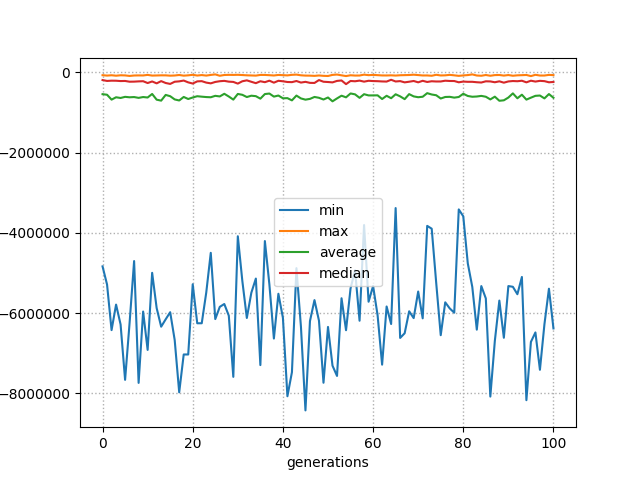
\includegraphics[width=\linewidth]{figures/TTP_eil51_n50_random.png}
    \caption{Resultados obtenidos en eil51\_n50}
    \label{figure:51_random}
\end{figure}

\begin{figure}[htbp!]
    \centering
    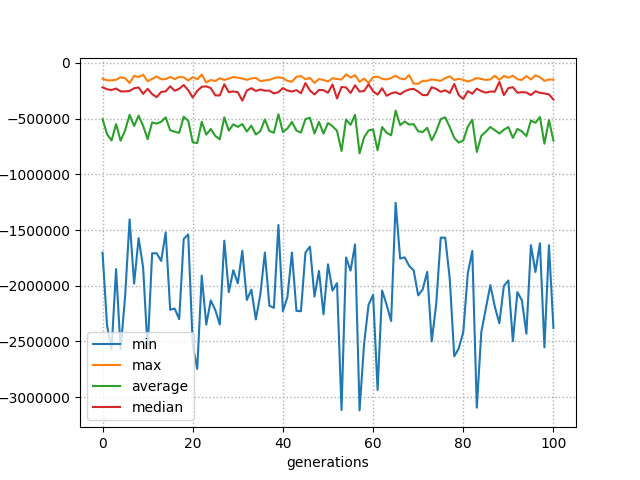
\includegraphics[width=\linewidth]{figures/ttp_eil76_random.png}
    \caption{Resultados obtenidos en eil76\_n75}
    \label{figure:76_random}
\end{figure}

\subsection{Seleccion por Torneo}
En vista de la variabilidad de los resultados se usa un operador que  ejerce mayor presión
a las poblaciones para forzarlas a mantener las buenas parejas, los resultados obtenidos se 
observan en la figura \ref{figure:51_torneum} y a tabla \ref{table:results_t}:

\begin{table}[htpb]
    \centering
    \begin{tabular}{|c|c|c|c|c|}
        \hline
        Problema & $\bar{x}$ & $\sigma_{\bar{x}}$ & mediana & $\sigma_{med}$ \\
        \hline
        eil51 n50 & -375814.18 & 253414.55 & -268596.97 & 275881.97 \\
        \hline
        eil76 n75 & -698416.9233 & 943446.0945 & -329127.2032 & 1029834.5280 \\
        \hline
    \end{tabular}
    \caption{Resumen estadistico selección por torneo}
    \label{table:results_t}
\end{table}

\begin{figure}[htbp!]
    \centering
    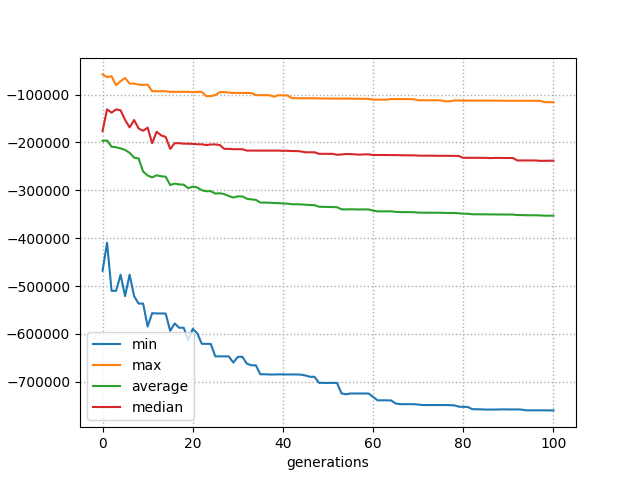
\includegraphics[width=\linewidth]{figures/TTP_eil51_n50_tournament.png}
    \caption{Resultados obtenidos en eil51\_n50}
    \label{figure:51_torneum}
\end{figure}

\begin{figure}[htbp!]
    \centering
    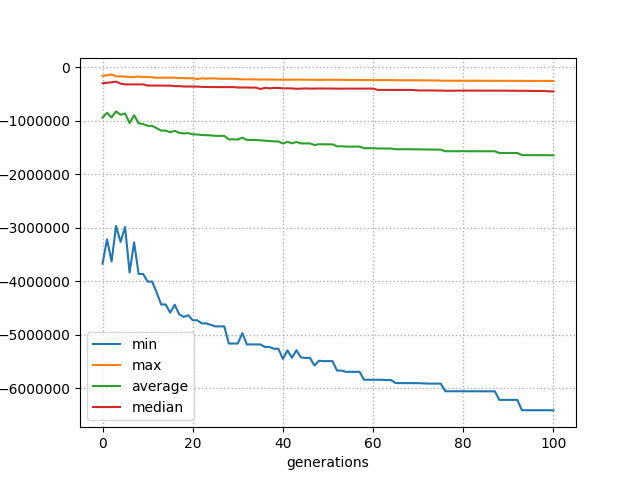
\includegraphics[width=\linewidth]{figures/ttp_eil76_tournament.png}
    \caption{Resultados obtenidos en eil76\_n75}
    \label{figure:76_torneum}
\end{figure}

De estos experimentos se puede evidenciar que al ejercer menos presion selectiva se obtienen
malos resultados en promedio, como se ve en las figuras \ref{figure:51_random} y \ref{figure:76_random}
, sin embargo las 
buenas soluciones son mucho mejores que las mejores soluciones resultantes de aplicar mayor,
presión. Sin embargo al hacer esto se obtiene una mayor consistencia en los resultados y un 
mejor resultado medio.

\section{Conclusiones}
El enfoque CoEvolutivo propuesto en este articulo brinda una buena forma de abordar el problema 
del ladron viajero, sin embargo es necesario balancear de manera correcta los operadores de cada
una de las poblaciones para poder encontrar mejores y mas consistentes soluciones. También es 
posible intentar ejercer mayor control sobre el cambio de amigo para poder mantener
consistencia en el rendimeinto de cada agente.


\begin{thebibliography}{X}
    \item Bonyadi, Michalewicz, Barone. The travelling thief problem: the first step in the
    transition from theoretical problems to realistic problems. \url{https://cs.adelaide.edu.au/~zbyszek/Papers/TTP.pdf}  
    \item Gomez, Garcia, Silva. COFRE: A FUZZY RULE COEVOLUTIONARY APPROACH FOR 
    MULTICLASS CLASSIFICATION PROBLEMS. \url{http://www.dis.unal.edu.co/~jgomezpe/docs/papers/cofre.pdf}
    \item Rodriguez, Gomez. Solución de problemas tipo Flow-Shop mediante algoritmos evolutivos.
    \url {http://bdigital.unal.edu.co/12916/}
    \item TTP problem instances. \url{https://cs.adelaide.edu.au/~optlog/CEC2014COMP_InstancesNew/}
    \item Wu, Polyakovhyi, Wawner, Newman. Evolutionary Computation plus Dynamic Programming for the
    Bi-Objective Travelling Thief Problem. \url{https://cs.adelaide.edu.au/~markus/pub/2018gecco-emottp.pdf}   
\end{thebibliography}

\end{document}